\newpage
\section{Приложение A. Устройство для измерения угла положения и линейного перемещения контролируемого объекта ИЗ №2780031}\label{sec:applicationA}
\begin{figure}[!h]
    \centering
    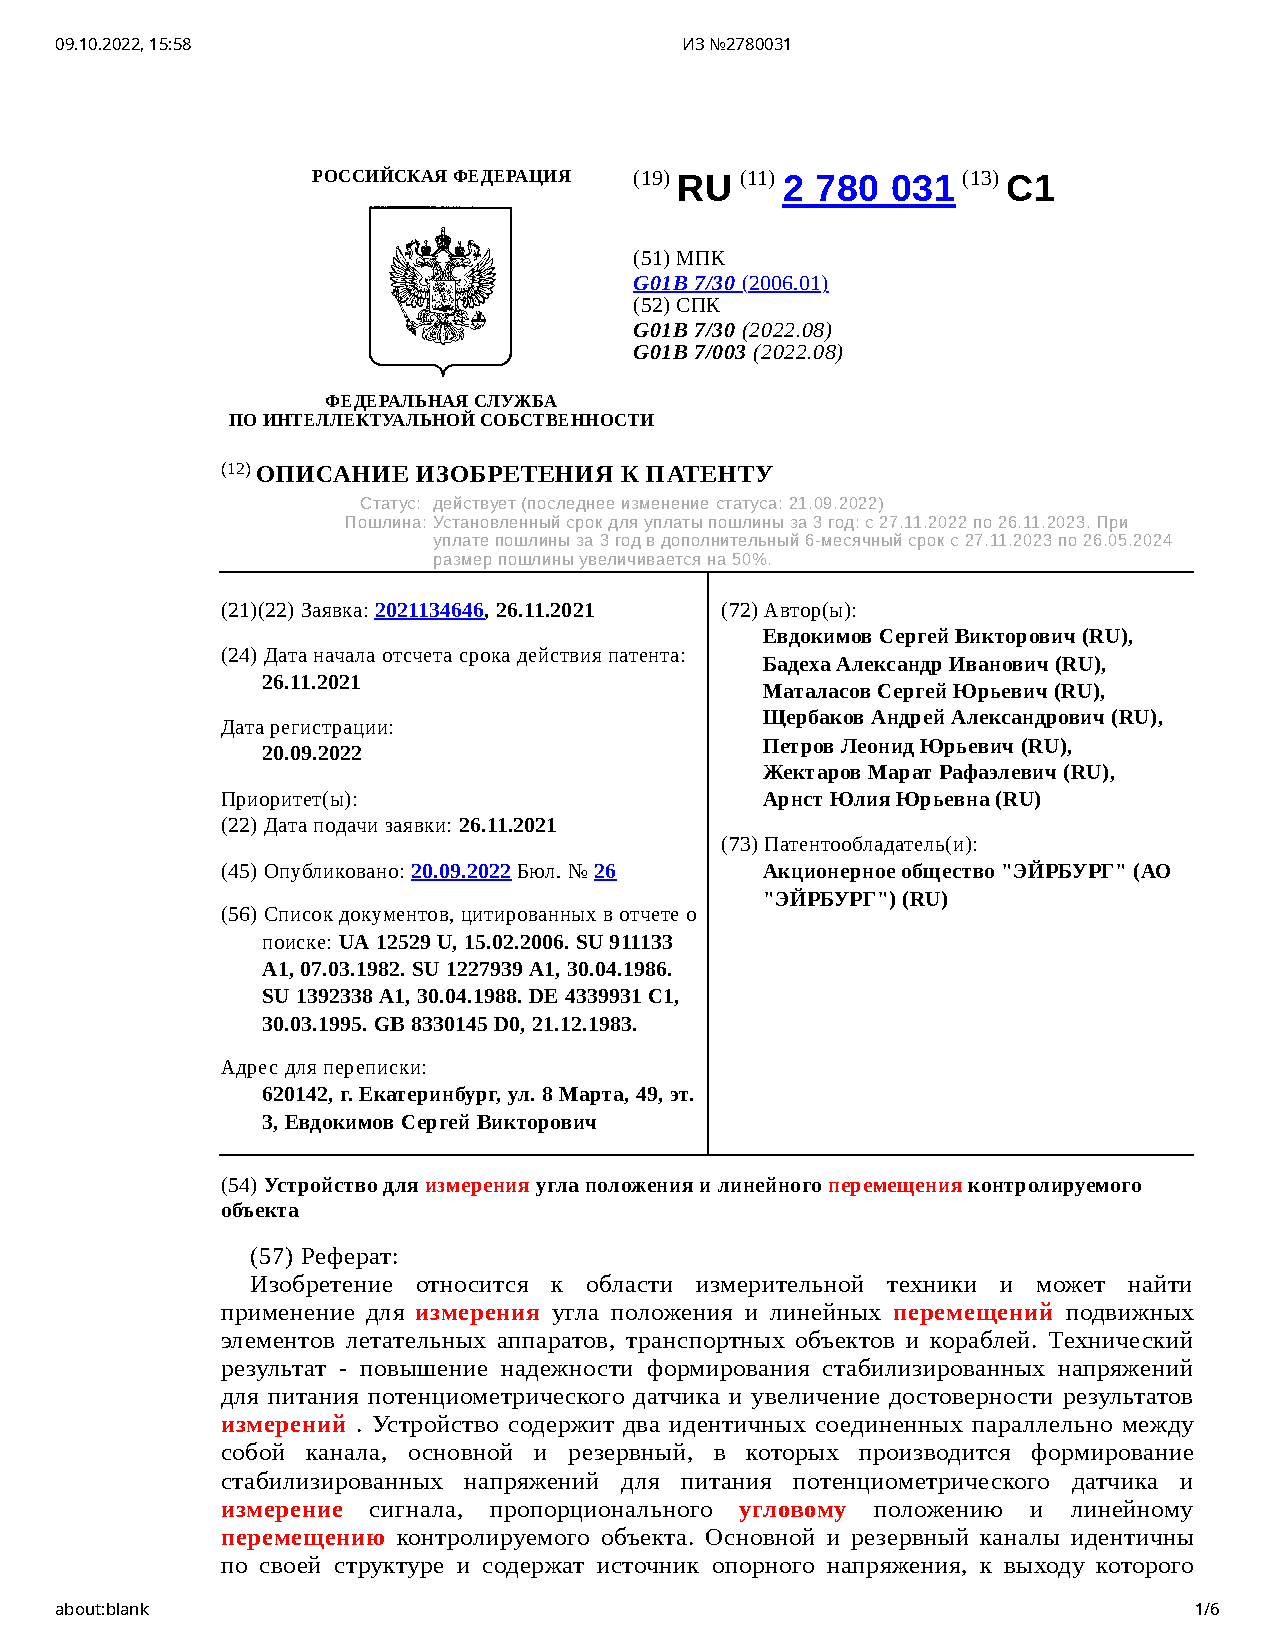
\includepdf[pages=1,width=1.1\textwidth]{pdf/2.pdf}
    \label{fig:app2.1}
\end{figure}
\newpage
\begin{figure}[!h]
    \centering
    \includepdf[pages=2,width=1.1\textwidth]{pdf/2.pdf}
    \label{fig:app2.2}
\end{figure}
\newpage

\begin{figure}[!h]
    \centering
    \includepdf[pages=3,width=1.1\textwidth]{pdf/2.pdf}
    \label{fig:app2.3}
\end{figure}
\newpage

\begin{figure}[!h]
    \centering
    \includepdf[pages=4,width=1.1\textwidth]{pdf/2.pdf}
    \label{fig:app2.4}
\end{figure}
\newpage

\begin{figure}[!h]
    \centering
    \includepdf[pages=5,width=1.1\textwidth]{pdf/2.pdf}
    \label{fig:app2.5}
\end{figure}
\newpage

\begin{figure}[!h]
    \centering
    \includepdf[pages=6,width=1.1\textwidth]{pdf/2.pdf}
    \label{fig:app2.6}
\end{figure}
\newpage

\section{Приложение Б. Преобразователь угловых перемещений ПМ №175216}\label{sec:applicationB}

\begin{figure}[!h]
    \centering
    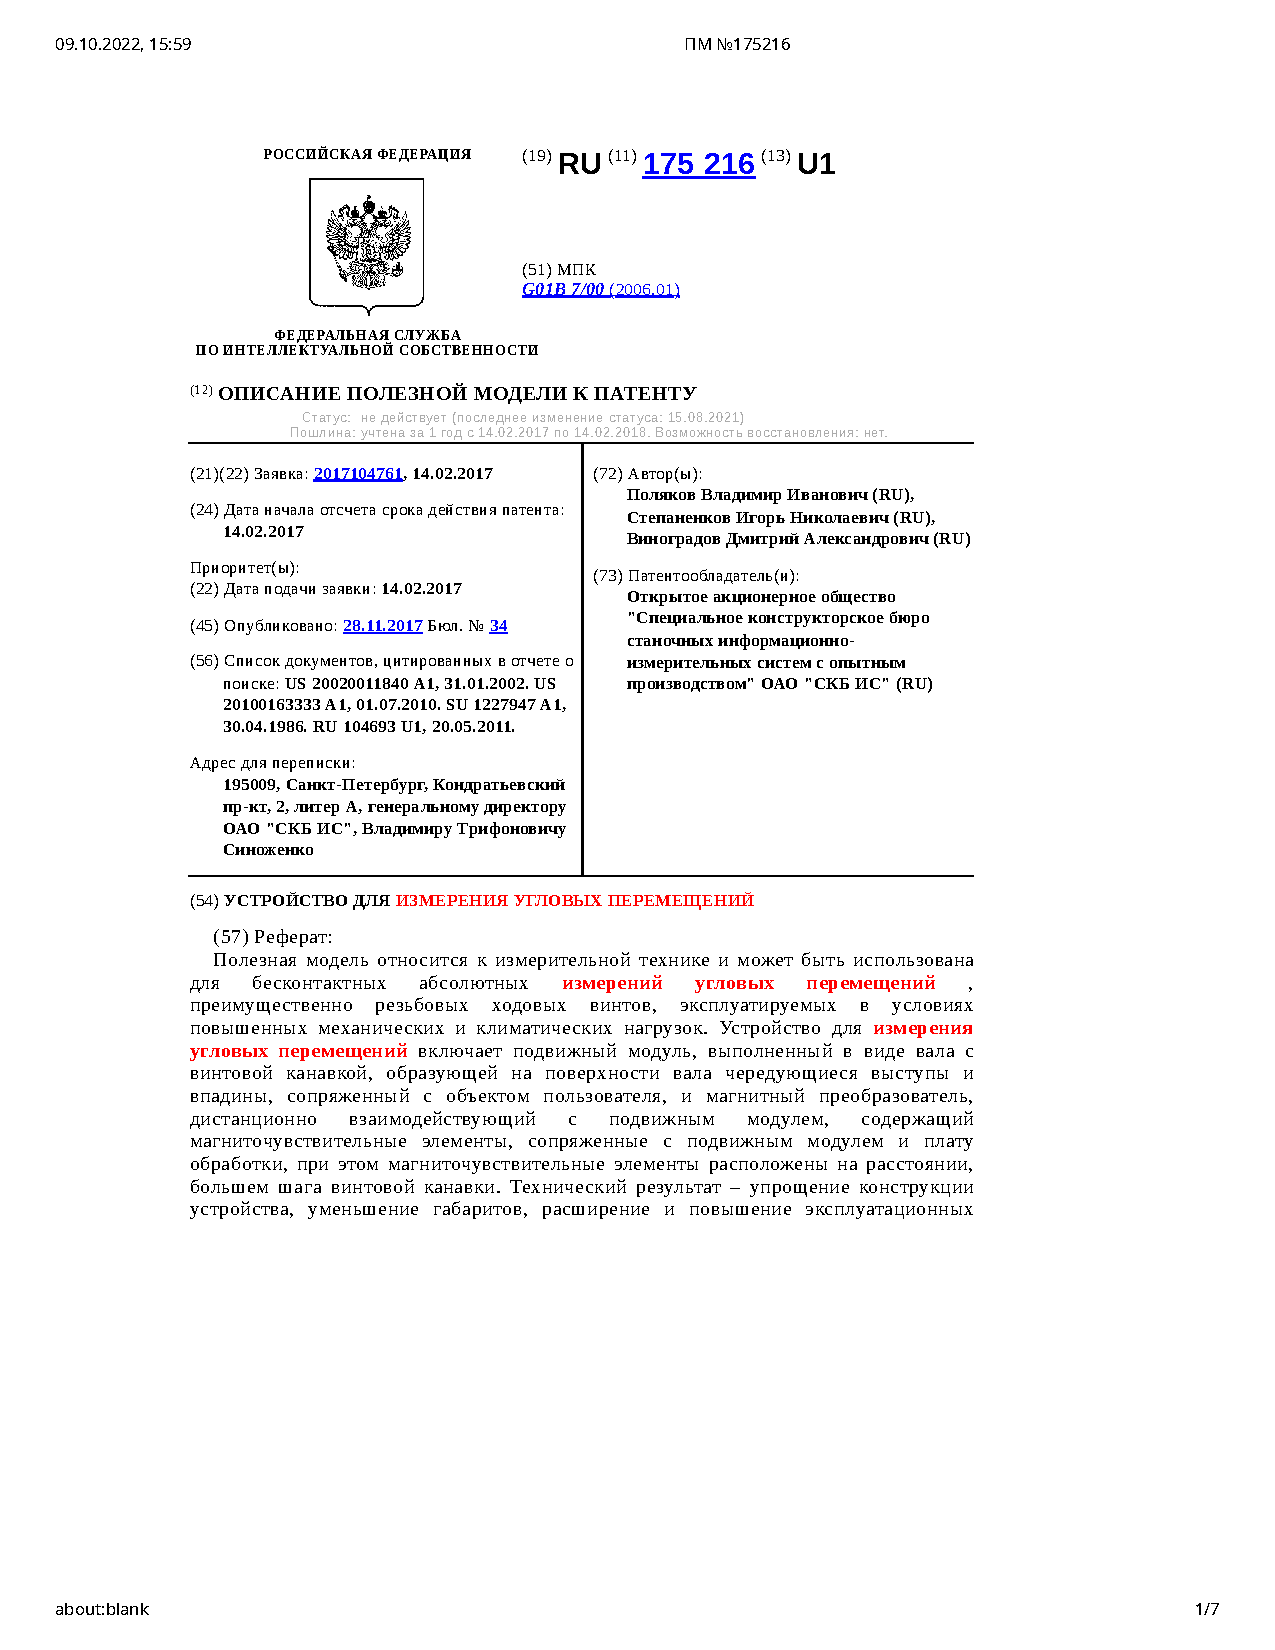
\includepdf[pages=1,width=1.1\textwidth]{pdf/3.pdf}
    \label{fig:app3.1}
\end{figure}
\newpage
\begin{figure}[!h]
    \centering
    \includepdf[pages=2,width=1.1\textwidth]{pdf/3.pdf}
    \label{fig:app3.2}
\end{figure}
\newpage

\begin{figure}[!h]
    \centering
    \includepdf[pages=3,width=1.1\textwidth]{pdf/3.pdf}
    \label{fig:app3.3}
\end{figure}
\newpage

\begin{figure}[!h]
    \centering
    \includepdf[pages=4,width=1.1\textwidth]{pdf/3.pdf}
    \label{fig:app3.4}
\end{figure}
\newpage

\begin{figure}[!h]
    \centering
    \includepdf[pages=5,width=1.1\textwidth]{pdf/3.pdf}
    \label{fig:app3.5}
\end{figure}
\newpage

\begin{figure}[!h]
    \centering
    \includepdf[pages=6,width=1.1\textwidth]{pdf/3.pdf}
    \label{fig:app3.6}
\end{figure}
\newpage

\begin{figure}[!h]
    \centering
    \includepdf[pages=7,width=1.1\textwidth]{pdf/3.pdf}
    \label{fig:app3.7}
\end{figure}
\newpage
\section{Приложение В. Преобразователь угловых перемещений ИЗ №2120105}\label{sec:applicationW}
\begin{figure}[!h]
    \centering
    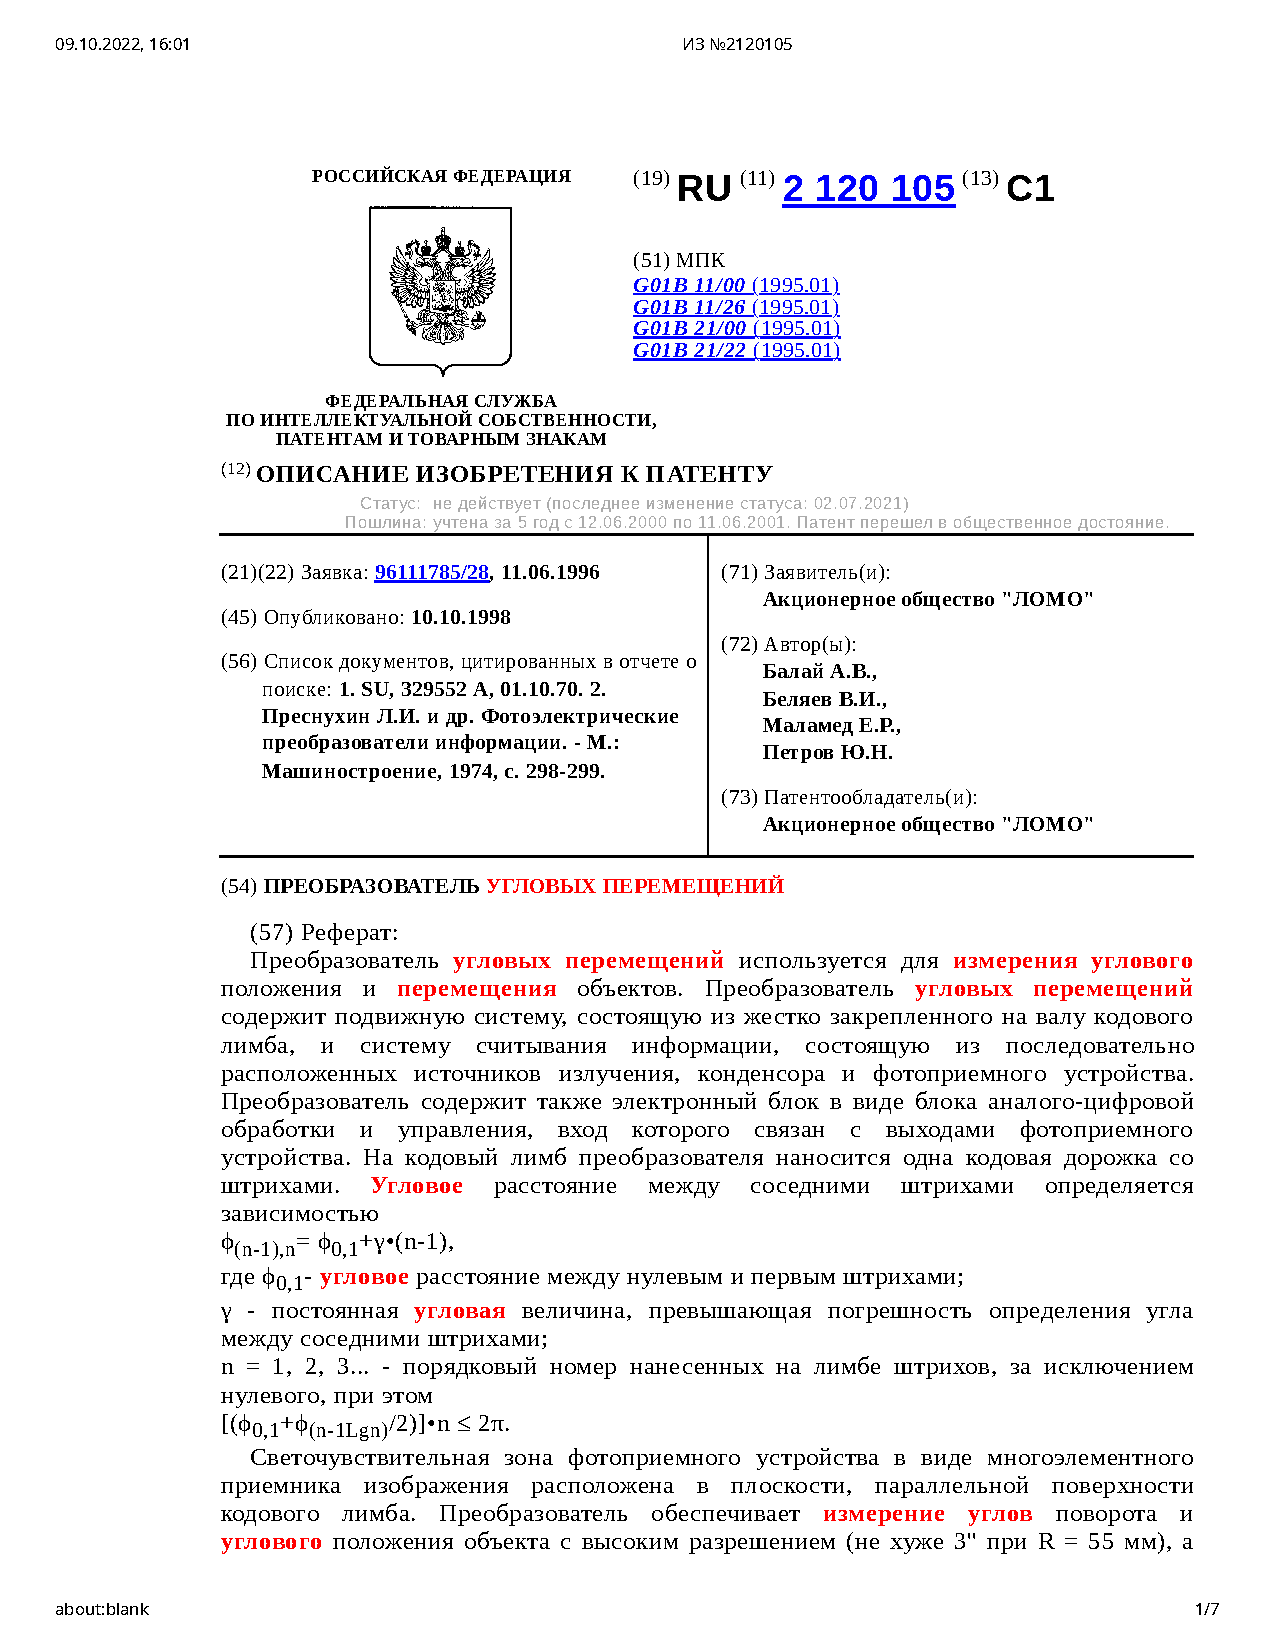
\includepdf[pages=1,width=1.1\textwidth]{pdf/1.pdf}
    \label{fig:app1.1}
\end{figure}
\newpage
\begin{figure}[!h]
    \centering
    \includepdf[pages=2,width=1.1\textwidth]{pdf/1.pdf}
    \label{fig:app1.2}
\end{figure}
\newpage

\begin{figure}[!h]
    \centering
    \includepdf[pages=3,width=1.1\textwidth]{pdf/1.pdf}
    \label{fig:app1.3}
\end{figure}
\newpage

\begin{figure}[!h]
    \centering
    \includepdf[pages=4,width=1.1\textwidth]{pdf/1.pdf}
    \label{fig:app1.4}
\end{figure}
\newpage

\begin{figure}[!h]
    \centering
    \includepdf[pages=5,width=1.1\textwidth]{pdf/1.pdf}
    \label{fig:app1.5}
\end{figure}
\newpage

\begin{figure}[!h]
    \centering
    \includepdf[pages=6,width=1.1\textwidth]{pdf/1.pdf}
    \label{fig:app1.6}
\end{figure}
\newpage

\begin{figure}[!h]
    \centering
    \includepdf[pages=7,width=1.1\textwidth]{pdf/1.pdf}
    \label{fig:app1.7}
\end{figure}

